\documentclass{beamer}
\usetheme{Berlin}

\usepackage{color}

\usepackage{tikz}
\usetikzlibrary{fit,positioning}



\begin{document}

\title{Prelim Exam}
\author{Xi Tan}
\date{April 15, 2016}
\maketitle

\section{Introduction}
\begin{frame}
\frametitle{Problem Description}
\begin{figure}[c]
  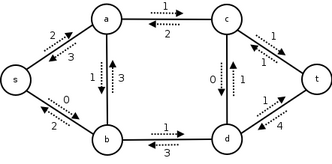
\includegraphics[width=0.5\textwidth]{figures/Network.png}
  \caption{An network consists of three elements: {\em{nodes}}, {\em{links}}, and {\em{messages}}. (Source: Wikipedia)}
\end{figure}

\begin{enumerate}
	\item Learn cluster structure of nodes;
    \item Model link intensities; 
    \item Model message contents.
\end{enumerate}

\end{frame}

\begin{frame}
\frametitle{Contributions}
\begin{enumerate}
	\item INMF extended previous parametric models to a non-parametric one, esp. learn \# clusters from data and can impose cluster structure constraints when learning;
    \item HP+GP+IRM extended the HP+IRM by introducing GPs to learn clusters and links from message contents;
    \item Both use CRP, MCMC to model and learn network structures;
    \item Propose to combine and generalize INMF and HP+GP+IRM and design a new (and efficient) algorithm to learn the model.
\end{enumerate}

\end{frame}

\begin{frame}
\frametitle{Table of Contents}
\begin{figure}[c]
  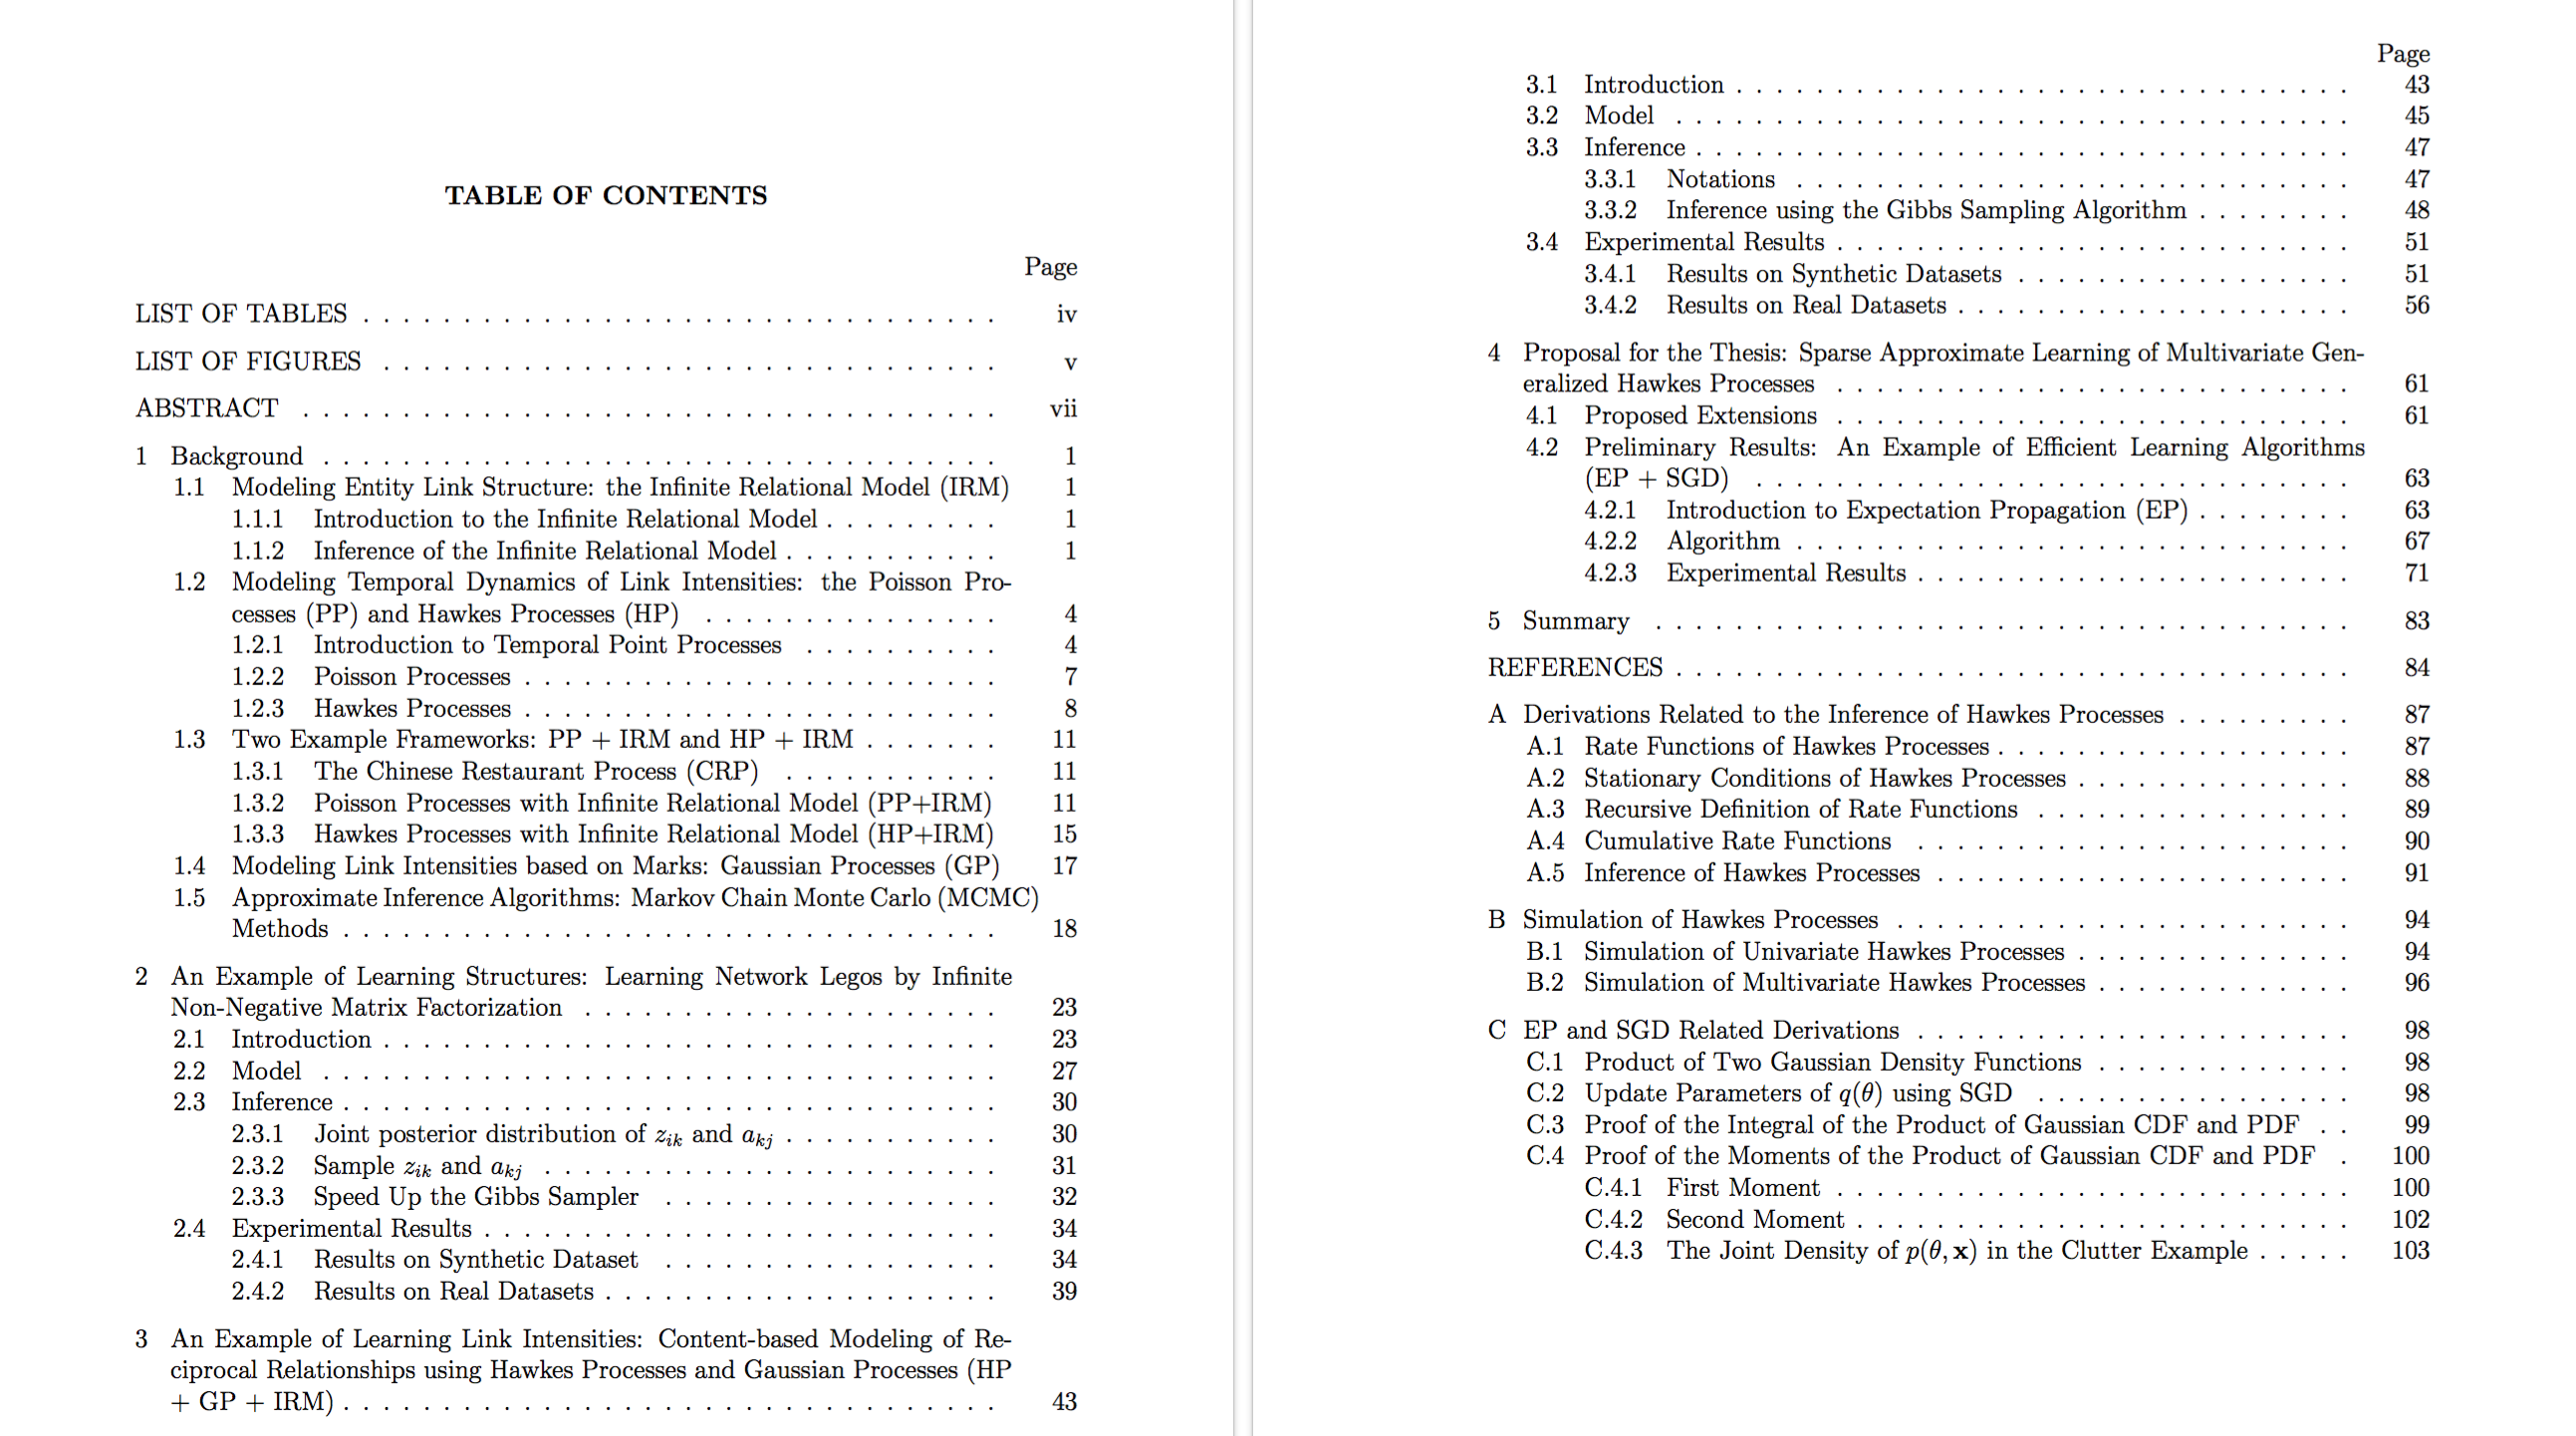
\includegraphics[width=\textwidth]{figures/toc.png}  
\end{figure}

\end{frame}

\section{Background}

\begin{frame}
\frametitle{The Chinese Restaurant Process (CRP)}
Suppose there are infinite number of round tables; the first customer chooses a new table with probability $1$; the $n^{th}$ customer with probability $\frac{1}{N-1+\alpha}$ chooses to sit with either any one of the previous $n-1$ customers, or a new table with probability $\frac{\alpha}{N-1+\alpha}$.

The joint probability is
\begin{align}
  p(\pi | \alpha) = \frac{\alpha^{|B|} \prod_{j=1}^{|B|} (|B_j|-1)!}{\prod_{j=1}^N (j-1+\alpha)} = \alpha^{|B|} \frac{\Gamma(\alpha)}{\Gamma(N+\alpha)} \prod_{j=1}^{|B|} \Gamma(|B_j|)
\end{align}
where $|B|$ is the total number of tables, and $(|B_j|-1)!$ is the factorial of $|B_j|-1$, the number of individuals in the $j^{th}$ table minus one.
\end{frame}


\begin{frame}
\frametitle{Infinite Relational Model (IRM)}
\begin{alignat}{3}
	\pi &| \alpha & &\sim CRP(\alpha)\\
	\lambda_{pq} &| \gamma & &\sim Beta(\gamma,\gamma) &\forall p,q \in range(\pi)\\
	e_{uv} &| \pi,\lambda_{\pi(u)\pi(v)} & &\sim Bernoulli(\lambda_{\pi(u)\pi(v)}) &\forall u,v \in V
\end{alignat}
\end{frame}


\begin{frame}
\frametitle{Point Processes}
\fontsize{6pt}{12}\selectfont
\begin{table}[ht]
\centering
    \begin{tabular}{| l | l |} \hline
    & \multicolumn{1}{|c|}{$\lambda(s)$: rate function at a specific time $s$}\\ \hline
    Homogeneous Poisson Processes & constant, independent of time \\ \hline
    Non-homogeneous Poisson Processes & constant, dependent on time \\ \hline
    Doubly Stochastic (Cox) Processes & independent random variable \\ \hline
    Self-exciting Hawkes Processes & random variable dependent on history of oneself\\ \hline
    Mutually-exciting Hawkes Processes & random variable dependent on history of others \\
    \hline    
    \end{tabular}
    \caption{Comparison of different point processes in terms of rate function types.}
\end{table}
\end{frame}


\begin{frame}
\frametitle{Hawkes Processes (1/2)}
\begin{figure}[ht]
  \centering
  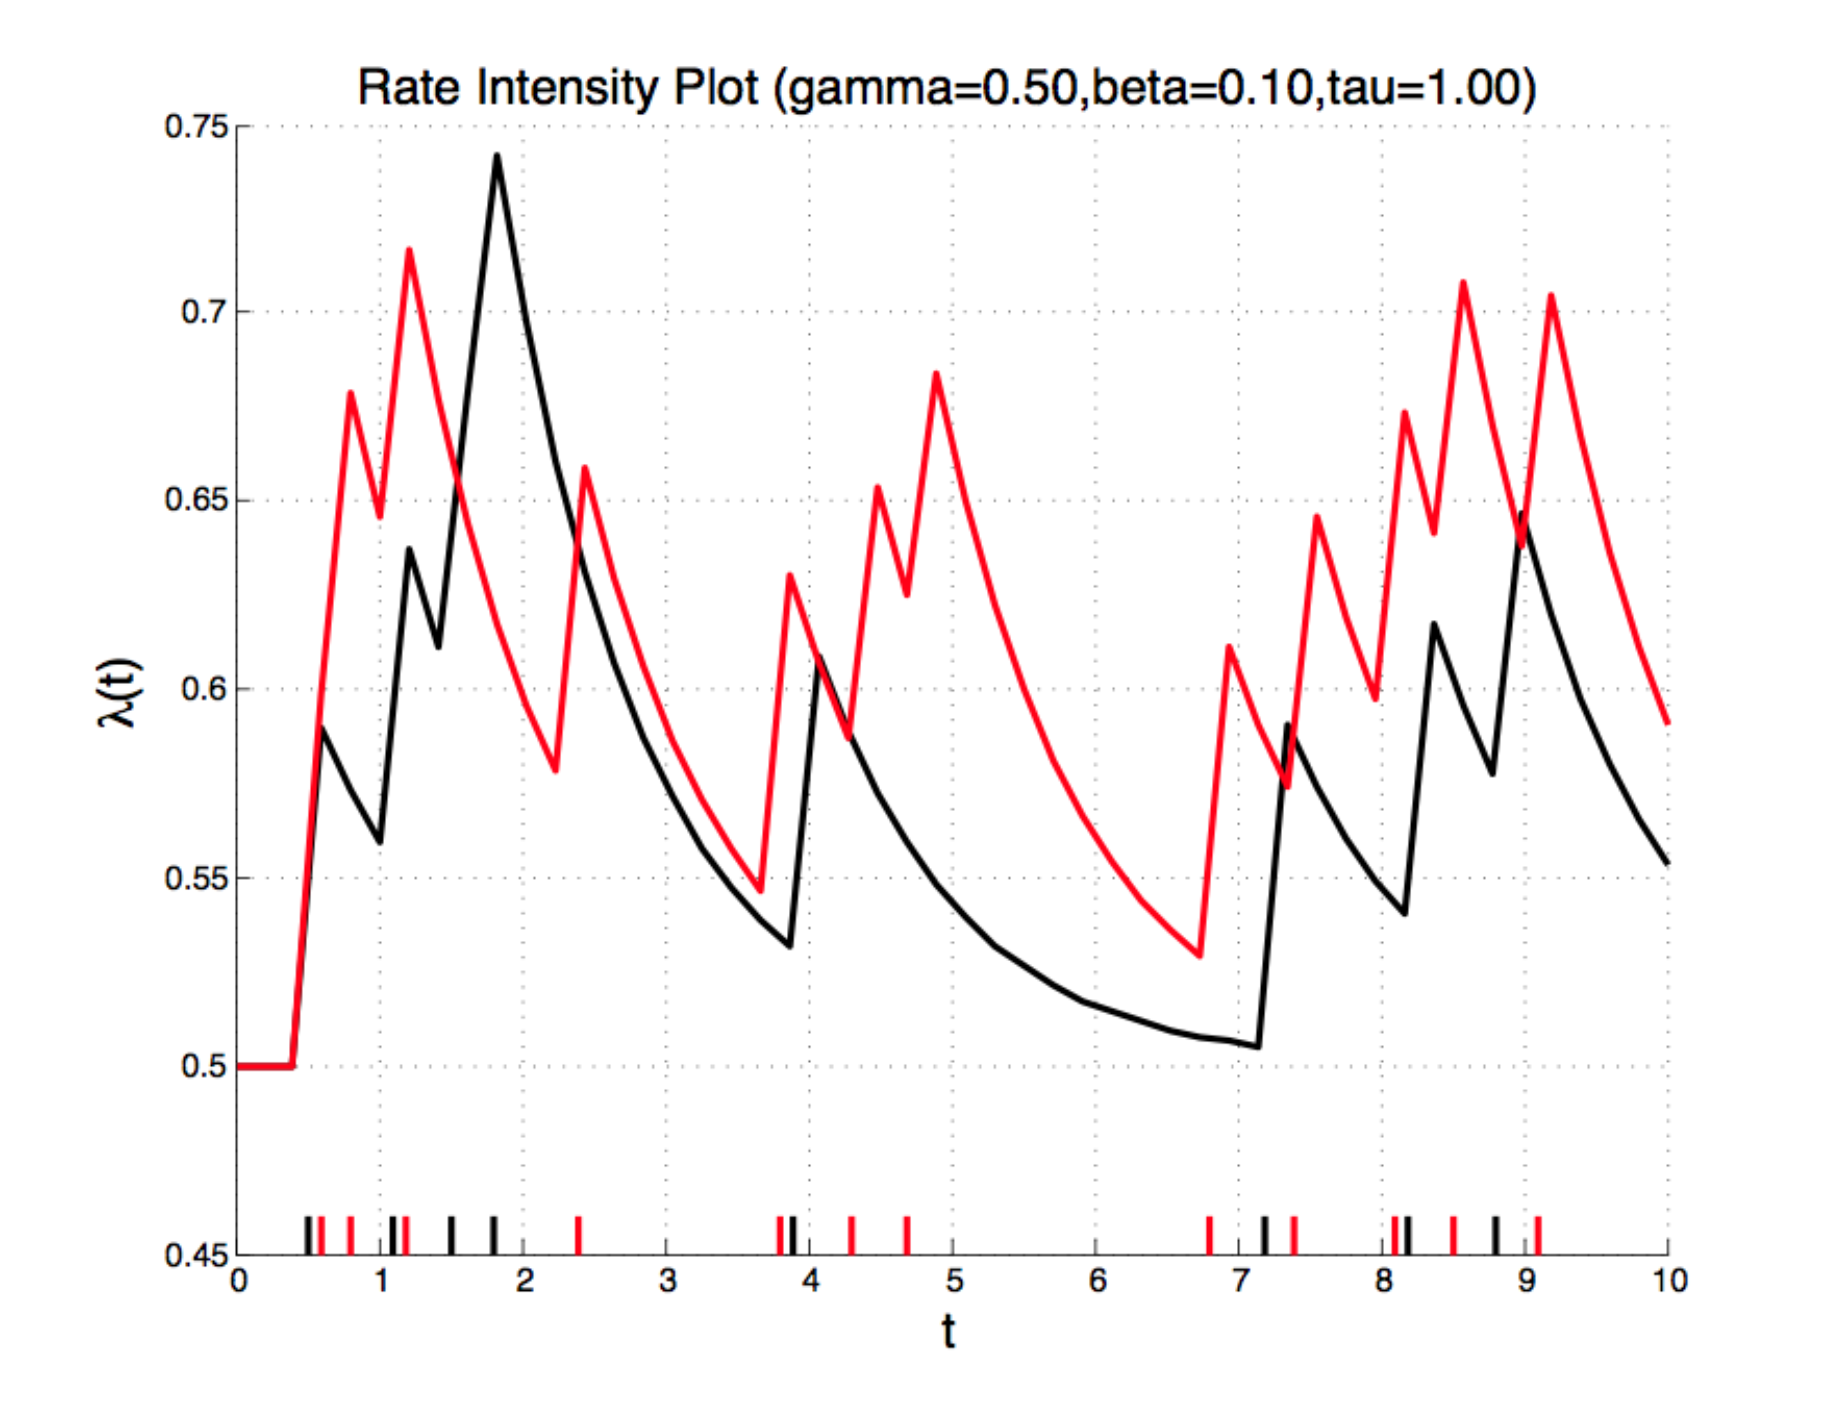
\includegraphics[width=0.4\textwidth]{figures/mutually-exciting}  
\end{figure}

\begin{alignat}{3}
  \lambda_{uv}(t) = \gamma + \beta \int_0^t e^{-\frac{t-s}{\tau}} dN_{vu}(s)  
\end{alignat}
If $\beta = 0$, Hawkes Processes reduce to (Homogeneous) Poisson Processes.
\end{frame}


\begin{frame}
\frametitle{Hawkes Processes (2/2)}
\begin{figure}[c]
	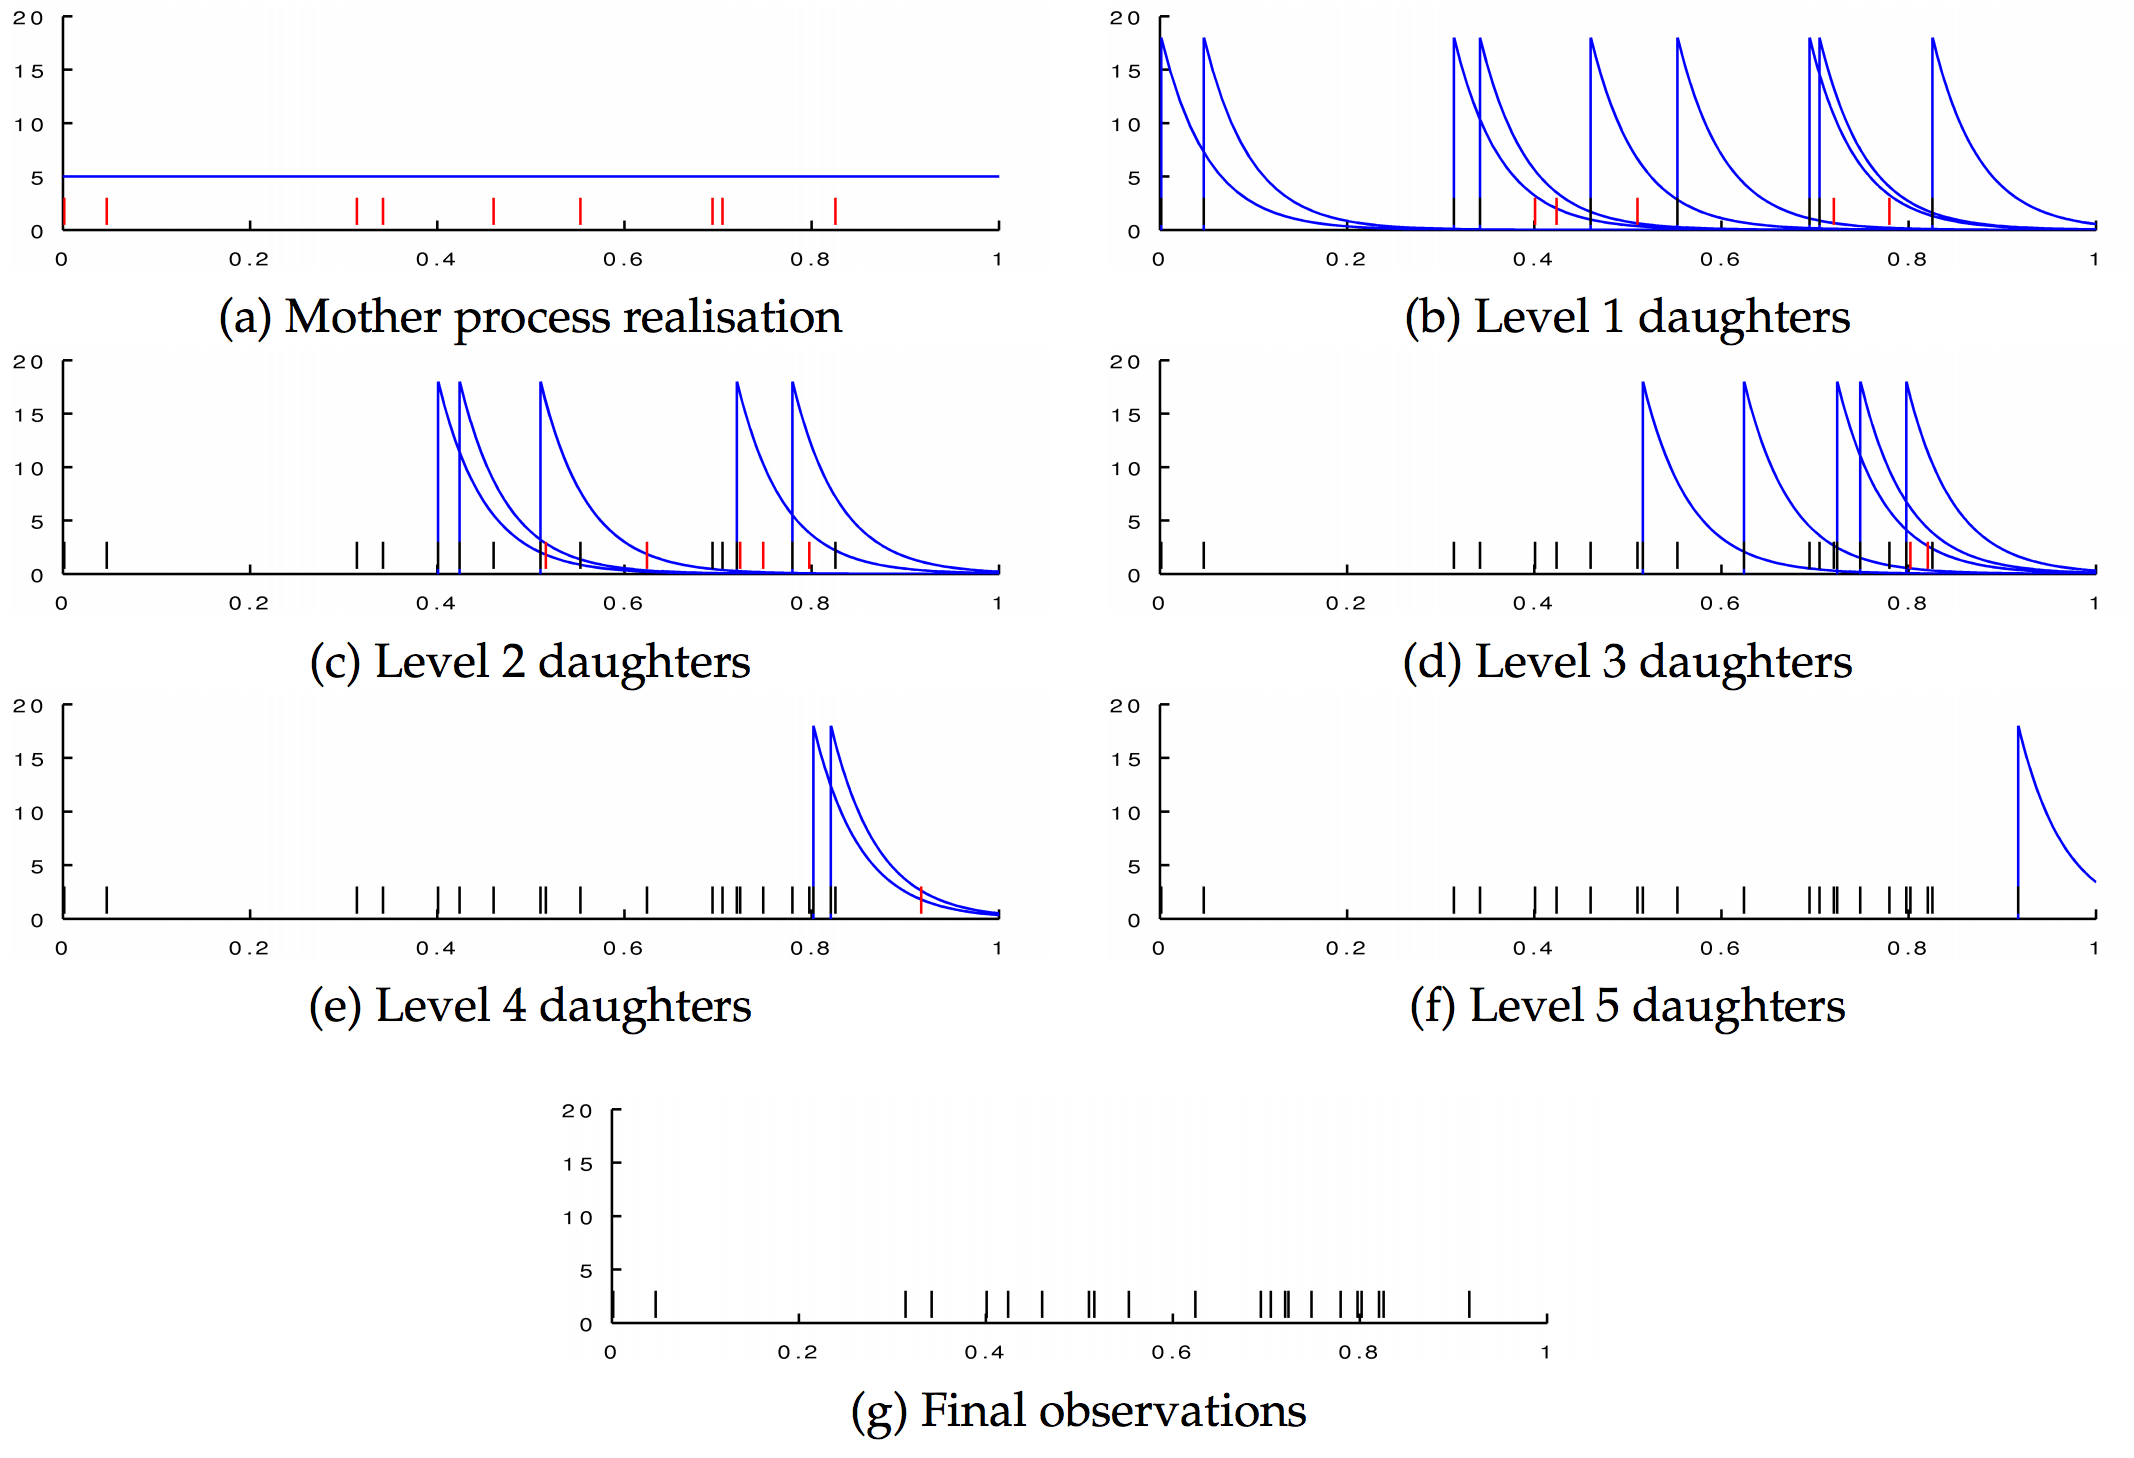
\includegraphics[width=0.8\textwidth]{figures/Hawkes_Imm}
\end{figure}
\end{frame}


\begin{frame}
\frametitle{Poisson IRM}
\begin{alignat}{3}
	\pi &| \alpha & &\sim CRP(\alpha)\\
	\lambda_{pq} &| \delta, \beta & &\sim Gamma(\delta,\beta) ~~~ \forall p,q \in range(\pi)\\
	N_{uv}(\cdot) &| \pi,\lambda_{\pi(u)\pi(v)} & &\sim PoissonProcess(\lambda_{\pi(u)\pi(v)}) ~~~ \forall u,v \in V
\end{alignat}
where $\pi$ is the assignment vector of length $|V|$, the total number of individuals; $\lambda_{pq}$ the rate of an individual in cluster $p$ sends a message to an individual in cluster $q$; $N_{uv}$ the number of messages sending from individuals $u$ to $v$.
\end{frame}


\begin{frame}
\frametitle{Hawkes IRM}
\begin{alignat}{3}
  &\pi | \alpha  \sim CRP(\alpha)\\
  &\lambda_{pq}(t) | \gamma_{pq},\beta_{pq},\tau_{pq}  = \gamma_{pq}n_pn_q ~~~ ~~~ + \nonumber\\ 
   &~~~ ~~~ ~~~ ~~~ ~~~\int_{-\infty}^t g_{pq}(t-s) dN_{qp}(s) \hspace{2mm}\forall p,q \in range(\pi)\\
  &N_{pq}(\cdot) | \lambda_{pq}  \sim HawkesProcess(\lambda_{pq})\\
  &N_{uv}(\cdot) | N_{\pi(u)\pi(v)}, \pi  \sim Thin(N_{\pi(u)\pi(v)}) \hspace{2mm}\forall u,v \in V
\end{alignat}
The operator $Thin$ refers to thinning; this  means distributing the atoms of $N_{pq}(\cdot)$ among each $N_{uv}(\cdot)$, such that $N_{pq} = \sum_{u,v}N_{u,v}(\cdot)$.
\end{frame}


\begin{frame}
\frametitle{Gaussian Processes (GP)}
The observed dataset $\DD = \{(x_1,y_1),\cdots,(x_n,y_n)\}$ and the point of interest $(x_*,y_*)$ are jointly Gaussian:
\begin{align}
	\begin{bmatrix}\by\\y_*\end{bmatrix} \sim \NN \left( \mathbf{0}, \begin{bmatrix}\K ~~~ \bk_*\\~\bk_*^T ~~k_{**}\end{bmatrix} \right)
\end{align}
where $\bk_* = k(x_*,x_i)$ and $k_{**} = k(x_*,x_*)$. The posterior of $y_*|\by$ is also Gaussian, with mean and variance
\begin{align}
	\mu &= \bk_*^T\K^{-1}\by\\
	\sigma^2 &= k_{**} - \bk_*^T\K^{-1}\bk_*
\end{align}

The inference of Gaussian Processes, largely depends on the covariance matrix and its inverse (the precision matrix), costs $O(n^2)$ space and $O(n^3)$ computations.
\end{frame}



\section{INMF}

\begin{frame}
\begin{center}
{\bf{Learning Network Legos by Infinite Non-negative Matrix Factorization (INMF)}}
\end{center}
\end{frame}

\begin{frame}
\frametitle{Problem Description}

\begin{figure}[c]
  \includegraphics[width=0.6\textwidth]{figures/network-lego-pipeline-cartoons.jpg}
\end{figure}

\begin{enumerate}
	\item Columns 1 and 2: A collection of response networks;
    \item Column 3: Want to learn network legos as building blocks;
    \item Column 4: Express response networks in terms of legos.
\end{enumerate}

\end{frame}

\begin{frame}
\frametitle{Matrix Representation}
\fontsize{6pt}{7.2}\selectfont
\begin{enumerate}
	\item Response Network $\Y_{N \times D}$
$$\Y = \bordermatrix{~ & Edge_1 & Edge_2 & \cdots & Edge_D\cr
                  RN_1 & 1 & 0 & \cdots & 1\cr
                  \cdots & \cdots & \cdots & \cdots & \cdots \cr
                  RN_N & 0 & 1 & \cdots & 1 \cr}_{N \times D}$$	
	\item Loading Matrix $\Z_{N \times K}$
$$\Z = \bordermatrix{~ & Lego_1 & Lego_2 & \cdots & Lego_K\cr
                  RN_1 & 1 & 0 & \cdots & 0\cr
                  \cdots & \cdots & \cdots & \cdots & \cdots \cr
                  RN_N & 1 & 1 & \cdots & 0 \cr}_{N \times K}$$	
	\item Lego Matrix $\A_{K \times D}$
$$\A = \bordermatrix{~ & Edge_1 & Edge_2 & \cdots & Edge_D\cr
                  Lego_1 & 1 & 0 & \cdots & 1\cr
                  \cdots & \cdots & \cdots & \cdots & \cdots \cr
                  Lego_K & 0 & 1 & \cdots & 1 \cr}_{K \times D}$$	
\end{enumerate}	

\end{frame}

\begin{frame}
\frametitle{Earlier Work}
This problem is essentially a matrix factorization problem, where a number of different methods have been developed, such as PCA, SVD, NMF, and etc. There are several limitations for the earlier work.
\begin{enumerate}
	\item Need to specify the number of legos $K$, which is actually unknown.
	\item When dealing with graphs, structure (connectivity, overlapness, and etc.) not take into account.
	\item We propose a new method called Infinite-NMF (INMF), which can learn $K$ automatically from the data, and find the best factorization under various structure constraints.
\end{enumerate}

\end{frame}


\subsection{Model}
\begin{frame}
\frametitle{Model Description}
\fontsize{6pt}{7.2}\selectfont

\begin{enumerate}
	\item The likelihood can be modeled as:
$$ P(\Y|\Z,\A) = p^{\|\Y\|_0 - \|\Y \oplus \hat\Y\|_0} (1-p)^{\|\Y \oplus \hat\Y\|_0} $$ where $\hat\Y = (\Z\A>0)$

	\item The prior for $\Z$ is an Indian Buffet Process (IBP) $$ P(\Z) = \frac{\alpha^{K_+}}{\prod_{h=1}^{2^N-1}K_h!}\exp\{-\alpha H_N\}\prod_{k=1}^{K_+}\frac{(N-m_k)!(m_k-1)!}{N!} $$

	\item The conditional for an edge $a_{kj}$ is described explicitly 
\begin{equation*}
		p(a_{kj}=1|\ba_{k,-j}) = \begin{cases}			
			0 & \text{if}\  a_{kj}\  \text{is NOT attached to $\ba_{k,-j}$} \\
			1 & \text{if}\  a_{kj}\  \text{is attached to $\ba_{k,-j}$ and a bridge} \\
			\frac{J1}{J1+J0} & \text{if $a_{kj}$ is attached to $\ba_{k,-j}$ and NOT a bridge} \\
		\end{cases}		
\end{equation*}
where $J1$ and $J0$ can be any structure measure when $a_{kj}=1$ and $a_{kj}=0$, respectively.
\end{enumerate}

\end{frame}

\subsection{Inference}
\begin{frame}
\frametitle{The MCMC Solution}
First of all, notice that $\Z$ and $\A$ are conditionally independent given the observation $\Y$

\begin{figure}[h]
\centering
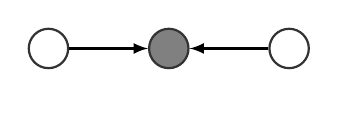
\begin{tikzpicture}
\tikzstyle{main}=[circle, minimum size = 5mm, thick, draw =black!80, node distance = 10mm]
\tikzstyle{connect}=[-latex, thick]
 \node[main, fill = white!100] (Z) [label=below:$\Z$] { };
 \node[main, fill=black!50] (Y) [right=of Z,label=below:$\Y$] { };
 \node[main] (A) [right=of Y,label=below:$\A$] { };

 \path (Z) edge [connect] (Y)
 (A) edge [connect] (Y);
\end{tikzpicture}
\end{figure}

So we can write

\fontsize{8pt}{7.2}\selectfont
\begin{align}	
	&p(z_{ik}, a_{kj}|\A_{-kj},\Z_{-ik},\Y) = p(z_{ik}|\A_{-kj},\Z_{-ik},\Y) p(a_{kj}|\A_{-kj},\Z,\Y) \\
	&p(z_{ik}|\A_{-kj},\Z_{-ik},\Y) \propto p(z_{ik}|\Z_{-ik}) \sum_{a_{kj}={0,1}} p(\Y|\Z, \A) p(a_{kj}|\A_{-kj}) \\
	&p(a_{kj}|\A_{-kj},\Z,\Y) \propto p(\Y|\Z, \A) p(a_{kj}|\A_{-kj})
\end{align}

\end{frame}

\begin{frame}
\frametitle{Two Tricks that Save Everything}
Without going into too much details, there is one simple yet extremely time consuming matrix operation that takes most of the computer time.

\vspace{0.1in}
Recall that we need to compute $\|\Y \oplus \hat\Y\|_0$, where $\hat\Y = (\Z\A > 0)$ involves

$$\Z_{N \times K} \times \A_{K \times D}$$ where $N \approx 20$, $K \approx 100$, and $D \approx 10K$.

\vspace{0.1in}
\fontsize{8pt}{7.2}\selectfont
We need to flip the value of just one element in $\A$, and re-evaluate this matrix product. This is repeated $N \times K + K \times D \approx 1M$ times in every iteration. If there are 200 iterations (reasonable number to converge), we are talking about $200 \times 20M \times 1M = 4,000,000,000,000,000$ multiplication operations here. That's why it took 3 weeks.


\end{frame}

\begin{frame}
\frametitle{Trick One: Local Update}
Trick One: If we flip the value of $A_{kj}$, only the $jth$ column of $\Z\A$ is affected. No need to compute the whole product, only local update.

\end{frame}

\begin{frame}
\begin{center}
  \begin{tabular}{ c | c | c || c | c}
    \hline
    $\hat y^{(k)}_{ij}$ & $\hat y^{(-k)}_{ij}$ & $y_{ij}$ & $\hat y_{ij} \oplus y_{ij}$ & $\hat y^{(-k)}_{ij} \oplus y_{ij}$ \\ \hline
    0 & 0 & 0 & $0 \oplus 0 = 0$ & $0 \oplus 0 = 0$ \\ \hline
    0 & 0 & 1 & $0 \oplus 1 = 1$ & $0 \oplus 1 = 1$ \\ \hline
    0 & 1 & 0 & $1 \oplus 0 = 1$ & $1 \oplus 0 = 1$ \\ \hline
    0 & 1 & 1 & $1 \oplus 1 = 0$ & $1 \oplus 1 = 0$ \\ \hline
    1 & 0 & 0 & $1 \oplus 0 = \color{red}{1}$ & $0 \oplus 0 = \color{red}{0}$ \\ \hline
    1 & 0 & 1 & $1 \oplus 1 = \color{red}{0}$ & $0 \oplus 1 = \color{red}{1}$ \\ \hline
    1 & 1 & 0 & $1 \oplus 0 = 1$ & $1 \oplus 0 = 1$ \\ \hline
    1 & 1 & 1 & $1 \oplus 1 = 0$ & $1 \oplus 1 = 0$ \\ \hline
  \end{tabular}
\end{center}

\fontsize{8pt}{7.2}\selectfont
\frametitle{Trick Two: The XOR Trick}
$\hat\Y^{(k)} = (\Z_k \A_k > 0)$ and $\hat\Y^{(-k)} = (\Z_{-k} \A_{-k} > 0)$, so $\hat\Y = \hat\Y^{(k)} \vee \hat\Y^{(-k)}$

Trick Two: We only need to update two cases when $\hat y^{(k)}_{ij} = 1$, otherwise, $\|\Y \oplus \hat\Y\|_0$ stays the same. This is $4$ times faster!

\end{frame}


\subsection{Results and Conclusion}
\begin{frame}
Results on Synthetic Datasets
\begin{figure}
  \centering
  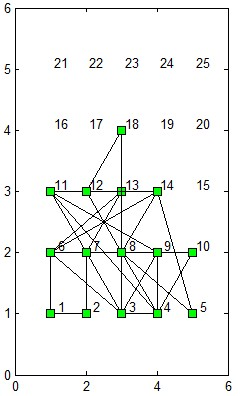
\includegraphics[width=.14\textwidth]{figures/true_X_1_2_6_7.jpg}
  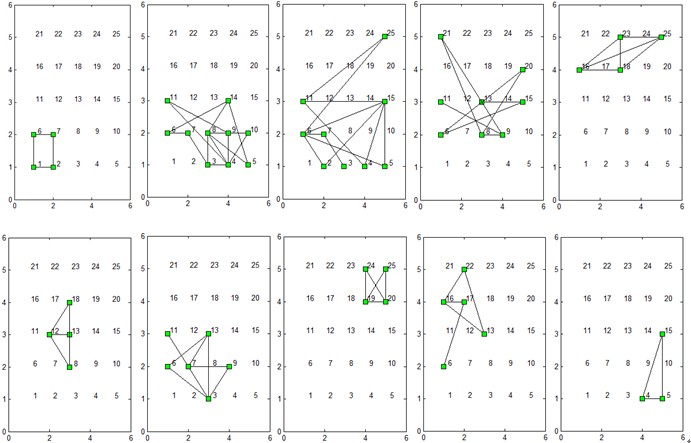
\includegraphics[width=.35\textwidth]{figures/trueBases.jpg}\\
  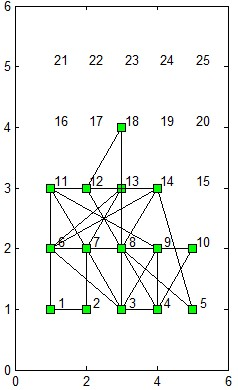
\includegraphics[width=.14\textwidth]{figures/predicted_X_1_2_6_7.jpg}
  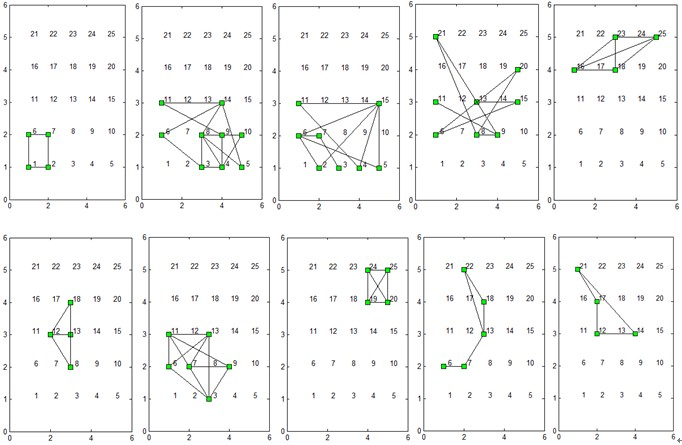
\includegraphics[width=.35\textwidth]{figures/predictedBases.jpg}
  \caption{Response network consists of bases 1, 2, 6, and 7; closewise from top left: true RN, true bases, predicted bases, predicted RN.}
\end{figure}

\end{frame}

\begin{frame}
Results on Real Datasets
\begin{table}[ht]
\centering
    \begin{tabular}{ | l | l | l |}
    \hline
      & Node Recovery & Edge Recovery \\ \hline
    response network \#1 & 81.25\% & 80.54\% \\ \hline     
    response network \#2 & 85.48\% & 87.45\% \\ \hline     
    response network \#3 & 91.25\% & 90.48\% \\ \hline     
    response network \#4 & 74.25\% & 68.78\% \\ \hline
    response network \#5 & 81.47\% & 80.48\% \\ \hline
    response network \#6 & 84.91\% & 85.01\% \\ \hline
    response network \#7 & 98.55\% & 97.15\% \\ \hline
    response network \#8 & 94.15\% & 90.71\% \\ \hline
    response network \#9 & 87.54\% & 84.15\% \\ \hline
    response network \#10 & 90.54\% & 89.45\% \\ \hline
    Average & 89.87\% & 88.23\% \\ \hline    
    \end{tabular}
    \caption{Summary statistics of the network legos for the ten response network dataset.}
    \label{table: summary for ten}
\end{table} 
\end{frame}

\section{HP+GP+IRM}
\begin{frame}
\begin{center}
{\bf{HP+GP+IRM: Content-based Modeling of Reciprocal Relationships using Hawkes and Gaussian Processes}}
\end{center}
\end{frame}

\subsection{Model}

\begin{frame}
\frametitle{Model Description}
We define the Hawkes process conditional rate function as:
\begin{alignat}{3}
	\lambda_{uv}(t) &= \gamma_{pq} + \int_0^t \beta_{uv} e^{-\frac{t-s}{\tau_{uv}}} dN_{vu}(s)
\end{alignat}
where $p = \pi^{-1}(u), q = \pi^{-1}(v)$ are the clusters individuals $u$ and $v$ belong to; and the triggering function $g_{uv}(\cdot)$ is defined as:
\begin{align}
	g_{uv}(\delta) &= \beta_{uv} e^{-\frac{\delta}{\tau_{uv}}}
\end{align}
\end{frame}

\begin{frame}
\frametitle{Model Description}
We propose to use two sets of Gaussian Process (GP) priors to address sources of inhomogeneity of the excitation functions $\beta_{uv}(\cdot)$, one for the significance of the message and one for the receptivity of the message:
\begin{align}
\beta_{uv}(s) =& e^{r_{u}(x_{vu}(s)) + s_{v}(x_{vu}(s))}\label{beta}
\end{align}
where
\begin{align}
  r_u(\cdot) \sim & \mathcal{GP}(0, k_r)\\
  s_v(\cdot) \sim & \mathcal{GP}(0, k_s)
\end{align}
$k_r$ and $k_s$ are radial basis function (RBF) kernels of the GPs. The exponential transformation is used to make sure that $\beta_{uv}(\cdot)$ is non-negative.

\end{frame}


\begin{frame}
\frametitle{Model Description}
\fontsize{10pt}{7.2}\selectfont
\begin{alignat}{3}
  &\pi | \alpha \sim CRP(\alpha)\\
  &\lambda_{uv}(t) | \gamma_{pq},\beta_{uv}(\cdot),\tau_{uv} = \gamma_{pq} + \int_{-\infty}^t \beta_{uv}(\XX_{vu}) e^{-\frac{t-s}{\tau_{uv}}} dN_{vu}(s)\hspace{1mm}\\
  &N_{uv}(\cdot) | \lambda_{uv} \sim HawkesProcess(\lambda_{uv})  
\end{alignat}
where $\XX_{vu} = \{x_{vu}(s)\}$ is the set of all messages sent from $v$ to $u$, and the cluster level excitation function $\beta_{pq}$ can be seen as an additive effect of $\beta_{uv}$:
\begin{align}
	\beta_{pq}(\XX_{qp}) =& \hspace{-5mm} \sum\limits_{\pi(u)=p, \pi(v)=q} \hspace{-5mm} \beta_{uv}(x_{vu}(s))
\end{align}

\end{frame}

\subsection{Inference}
\begin{frame}
\frametitle{Inference}
We use elliptical slice sampling to learn GP related quantities, e.g., $r_u, s_v$, and use slice sampling to learn other parameters.
\end{frame}

\begin{frame}
\frametitle{Synthetic Datasets: Two Individuals (1/3)}
\begin{figure}
  \centering  
	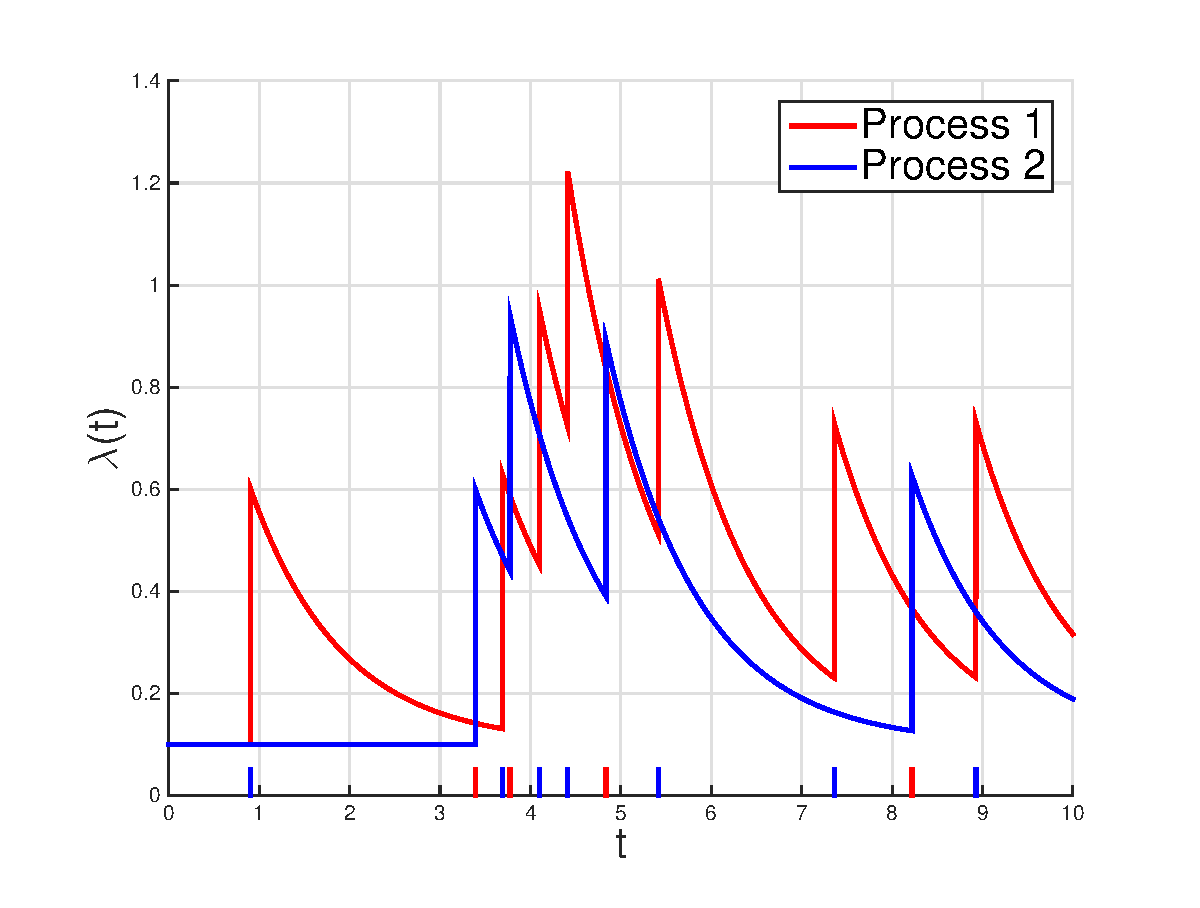
\includegraphics[width=0.4\textwidth]{figures/case1}
  \label{fi: example 1}
\end{figure}
In part (a), case 1 used a constant message content $x_{12}(t_i) = x_{21}(t'_i) = 1$ for all event times $t_i$ and $t'_i$, and a constant excitation function $\beta_{12}(x) = \beta_{21}(x) = x = 1$ for all messages.
\end{frame}

\subsection{Results}
\begin{frame}
\frametitle{Synthetic Datasets: Two Individuals (2/3)}
\begin{figure}
  \centering  
	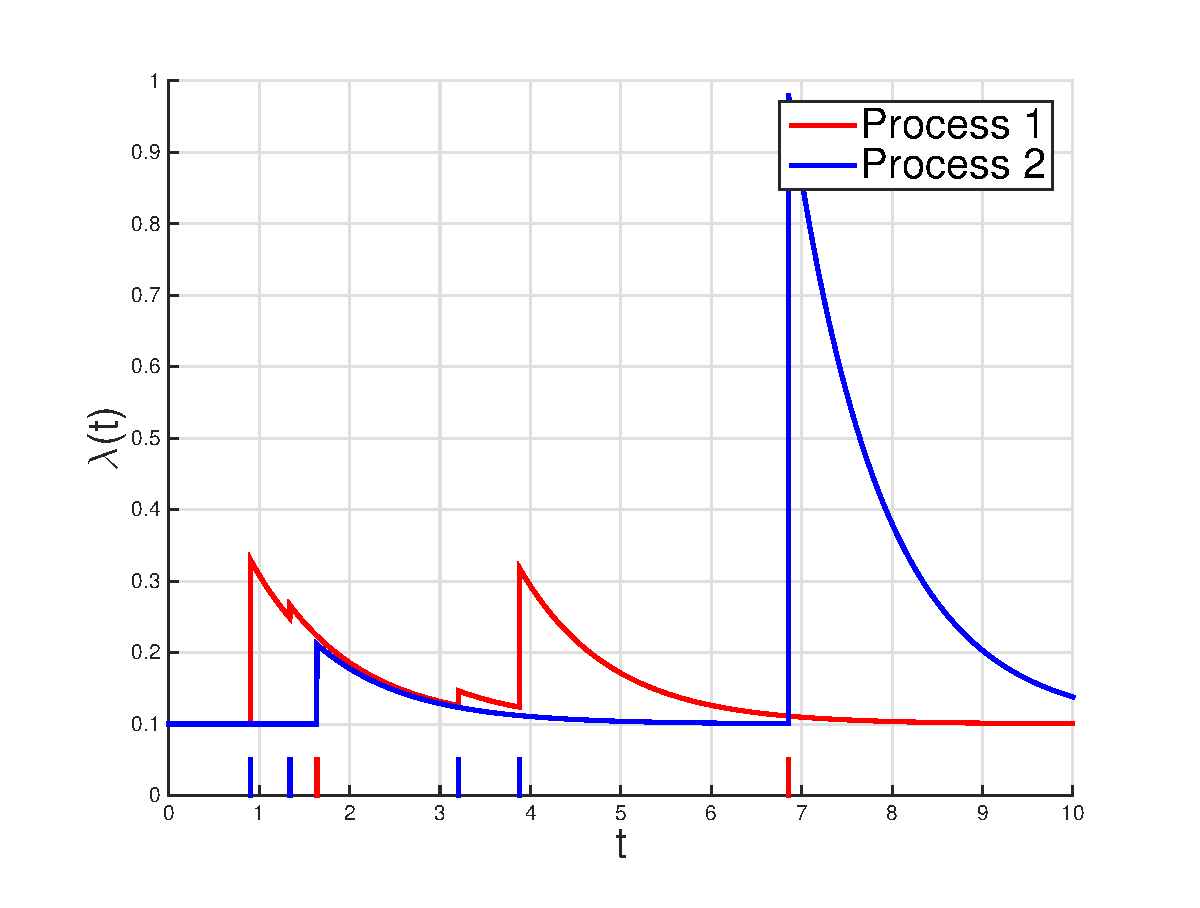
\includegraphics[width=0.4\textwidth]{figures/case2}
  \label{fi: example 1}
\end{figure}
In part (b), case 2 used the same settings as part (a), except for the introduction of variable message content, where both $x_{12}(t_i)$ and $x_{21}(t'_i)$ follow an exponential distribution $\exp(0.5)$, which can be thought of as different message entropy values at different event times $t_i$ and $t'_i$. We see that the jump sizes of both processes are no longer constant.
\end{frame}

\begin{frame}
\frametitle{Synthetic Datasets: Two Individuals (3/3)}
\begin{figure}
  \centering  
	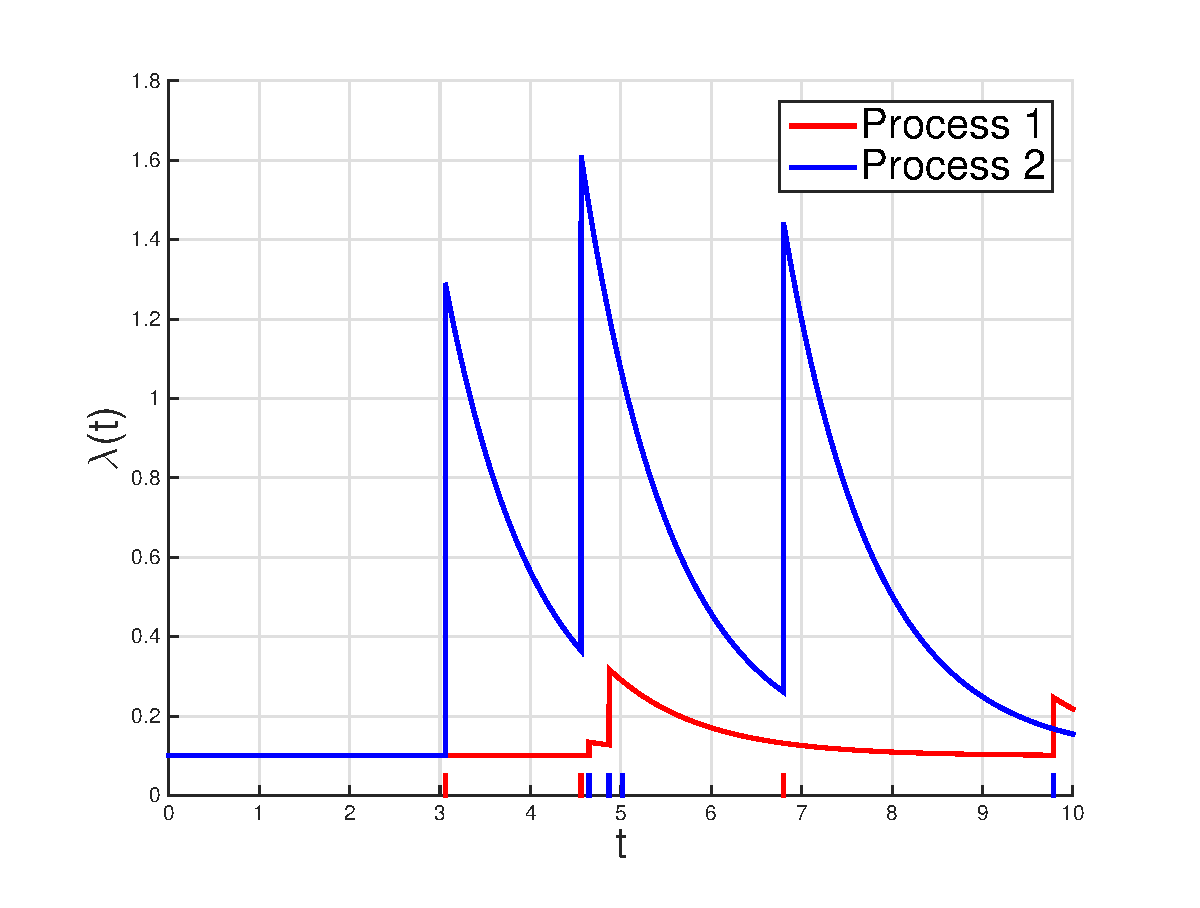
\includegraphics[width=0.4\textwidth]{figures/case3}
  \label{fi: example 1}
\end{figure}
In part (c), case 3 further introduced non-constant $\beta_{uv}(\cdot)$, with all other settings being the same as in case 2, but $\beta_{12}(t_i) = e^{2sin(x_{21}(t_i)) + 1.5log(x_{21}(t_i))}$ and $\beta_{21}(t'_i) = e^{0.1cos(x_{12}(t'_i)) + 0.2\sqrt{x_{12}(t'_i)}}$.

\end{frame}


\begin{frame}
\frametitle{Synthetic Datasets: Two Individuals}
\begin{figure}
  \centering  
	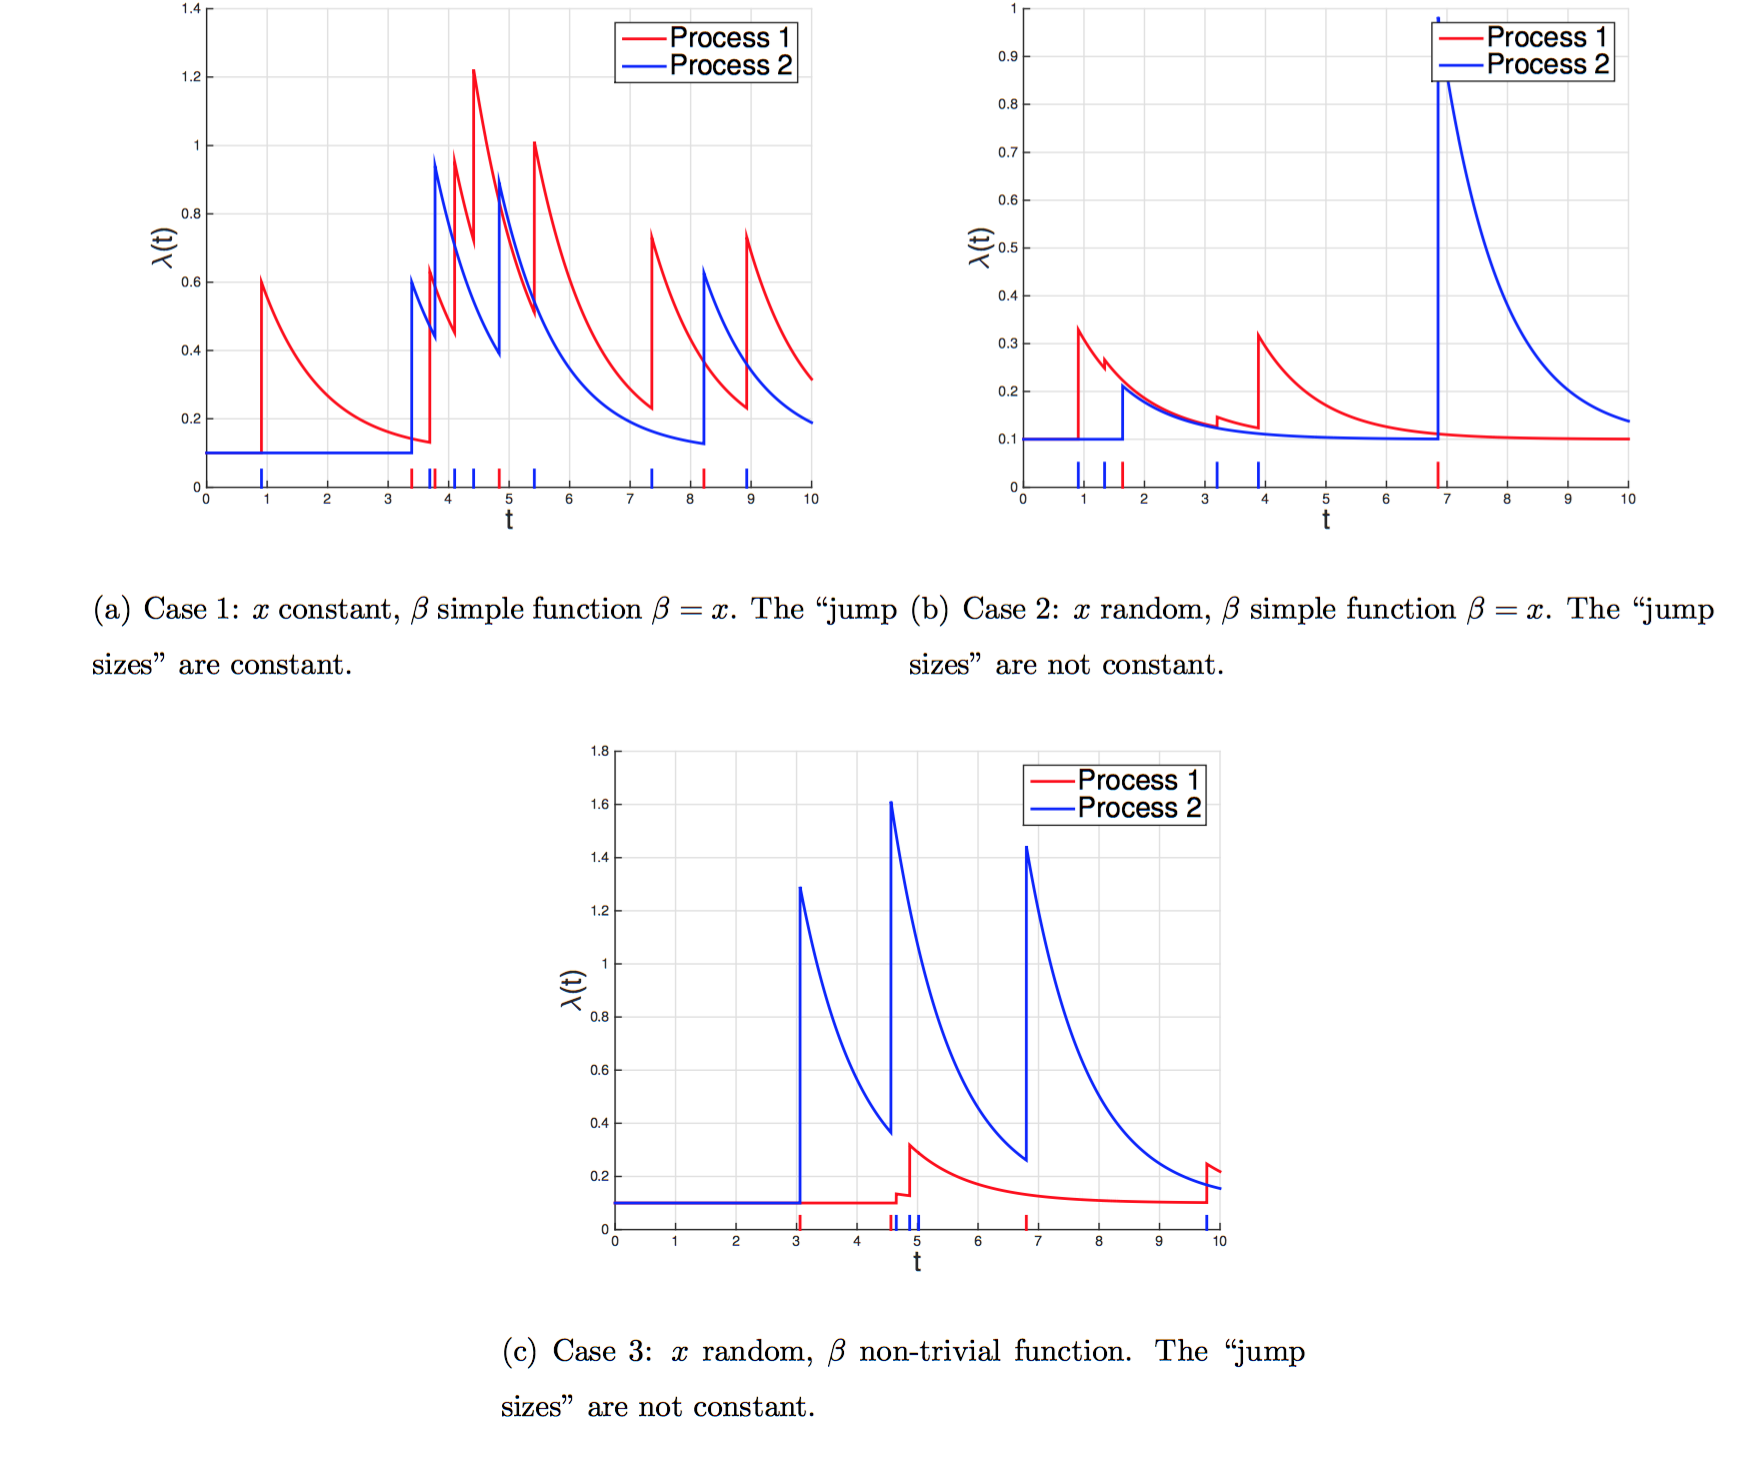
\includegraphics[width=0.7\textwidth]{figures/rate}
  \label{fi: example 1}
\end{figure}
\end{frame}


\begin{frame}
\frametitle{Synthetic Datasets: Two Individuals}
\begin{table}[ht]
\caption{Log likelihood comparison for the three-case synthetic data set}
\begin{center}
\begin{small}
\begin{sc}
\begin{tabular}{|r|c|c|c|}
\hline
%\belowspace
  & case 1  & case 2 & case 3\\
\hline
HP+GP+IRM & -21.88 & -13.41 & -10.86\\
\hline
HP+IRM & -22.97 & -35.53 & -82.78\\
\hline
Poisson + IRM & -72.31  & -89.73 & -126.33\\
\hline
HP & -129.37  & -238.94 & -192.78\\
\hline
Poisson & -127.83  & -182.76 & -187.23\\
\hline
\end{tabular}\label{synthetic training log  likelihood}
\end{sc}
\end{small}
\end{center}
\end{table}
\end{frame}


\begin{frame}
\frametitle{Synthetic Datasets: Three Individuals}
\begin{figure}
  \centering  
	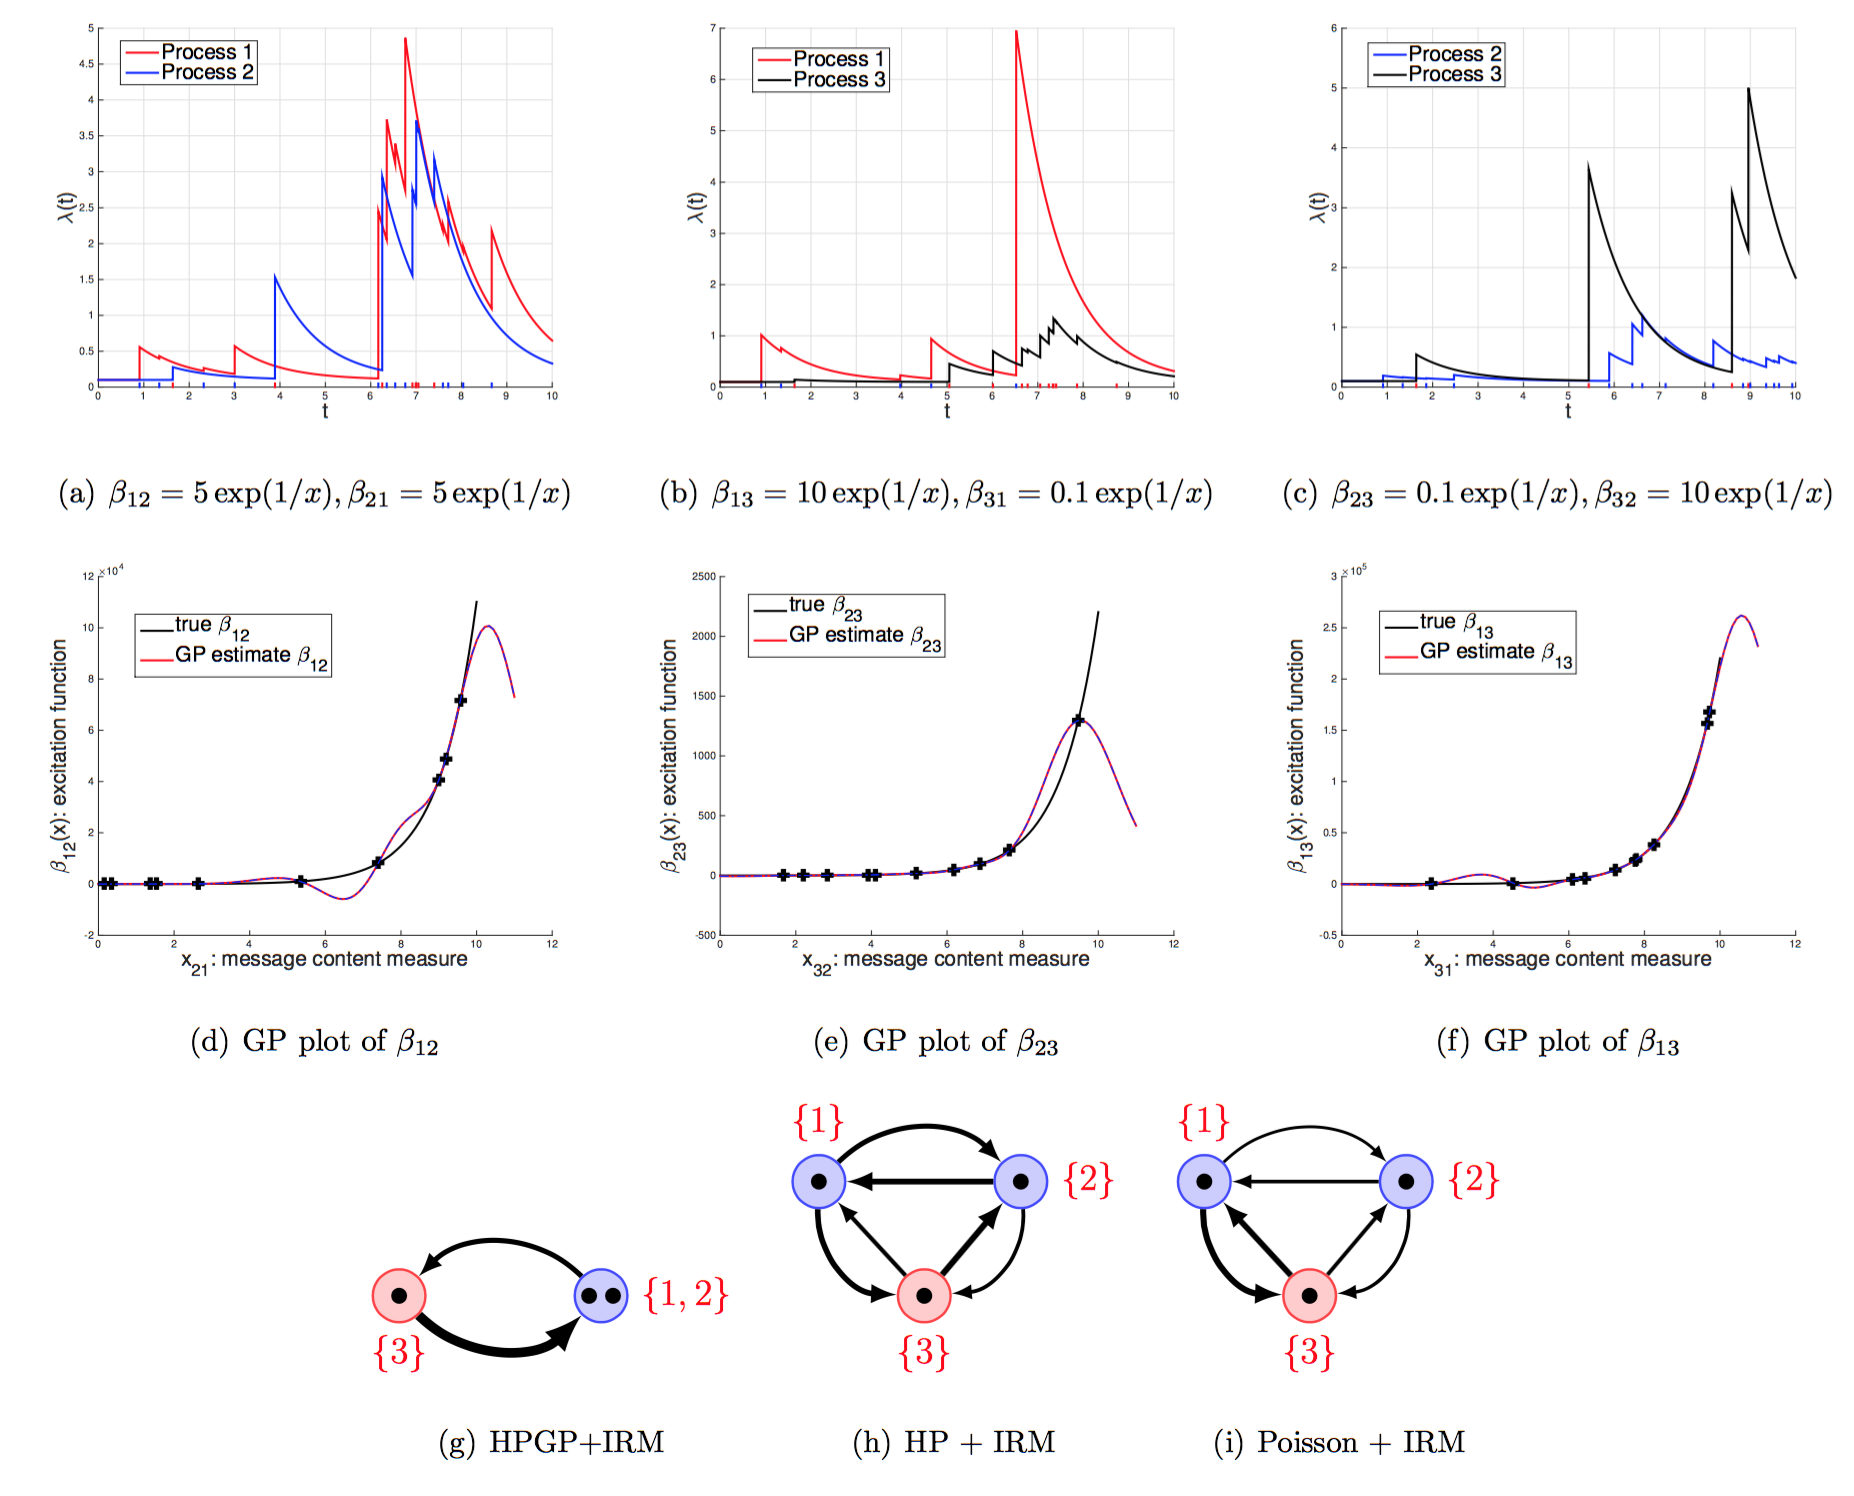
\includegraphics[width=0.75\textwidth]{figures/example2}
  \label{fi: example 1}
\end{figure}
\end{frame}


\begin{frame}
\frametitle{Real Datasets}
\begin{figure}
  \centering  
	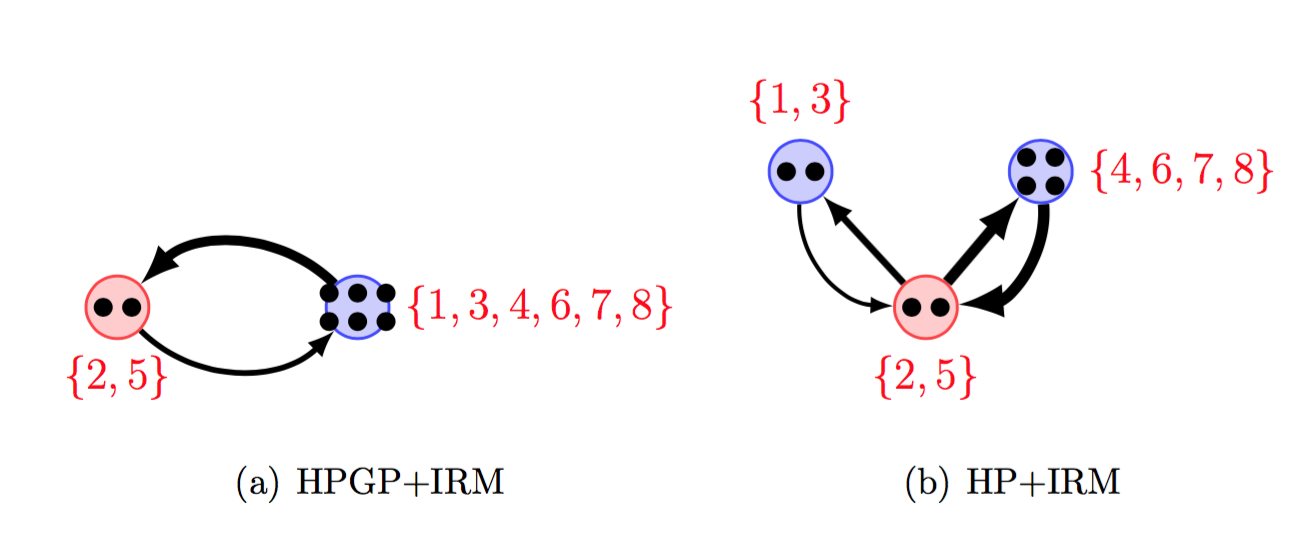
\includegraphics[width=0.75\textwidth]{figures/realdata}
  \caption{The data set used (\#33) is a lively family argument/discussion recorded at a vacation home in Falmouth, Massachusetts. There are eight participants, all relatives or close friends. Discussion centers around a disagreement Jennifer (\#2) is having with her mother Lisbeth (\#5).}
\end{figure}
\end{frame}


\section{Proposal}

\subsection{Sparse Multivariate Hawkes Processes}
\begin{frame}
\frametitle{Sparse Multivariate Hawkes Processes}
In the HP+GP+IRM framework, we can also impose desired constraints such as sparsity with multivariate Hawkes Processes:
\begin{align}
\lambda_u(t) = \gamma_{\pi^{-1}(u)} + \sum_{v=1}^{|V|} z_{uv} a_{uv} \int_{-\infty}^t \beta_{uv}(\XX_{vu}) e^{-\frac{t-s}{\tau_{uv}}} dN_{vu}(s)
\end{align}
where the binary adjacency matrix $\Z = \{z_{uv}\}$ and the non-negative weight matrix $\A = \{a_{uv}\}$ specify the structure and strength of the interaction network.
\end{frame}

\subsection{Generalized Hawkes Processes}
\begin{frame}
\frametitle{Generalized Hawkes Processes}
If we take a closer look at a realized Hawkes Process, especially a high-frequency one, we see that the rate function can be composed into a global ``trend'' and local ``fluctuations''. This observation is common in Finance, where ``trend'' and ``fluctuations'' are usually referred to as ``drift'' and ``volatility'', respectively. To model this two level structure, we may use the Generalized Hawkes Process, where the dynamics of the rate function can be written as:
\begin{align}
	d \lambda(t) = k(\lambda_{\infty}-\lambda(t)) dt + \delta dN_t + \sigma dW_t
\end{align}
where the added randomness $W = \{W_t: 0 \le t\}$ is a standard Brownian motion independent of $N_t$. The first two terms in the above equation capture the ``drift'' of the rate function and the last term captures the ``volatility'' of the rate function.
\end{frame}


\subsection{Efficient Learning Algorithms for Hawkes Processes}
\begin{frame}
\frametitle{Efficient Learning Algorithms for Hawkes Processes}
Recall the likelihood function of both Poisson Processes and Hawkes Processes (and many other Poisson related processes):
\begin{align}
  \LL(\lambda(t)|\HH) = \exp\left\{-\Lambda(0,T)\right\} \prod_{i=1}^n \lambda(t_i) \label{like}
\end{align}
This product form of likelihood fits right into the framework of EP.
\end{frame}

\begin{frame}
\frametitle{Other Possible Extensions}
Spectral analysis on Hawkes Processes may provide us with further insight from the frequency domain.

\vspace{0.1in}
Another perspective of learning Hawkes Processes is inspired by the ``drift'' and ``volatility'' observation of the rate function, and their ``immigrants'' and ``offspring'' representation. At the first level, we can learn the ``drift'' part (or the ``global'' picture, the ``trend'') of the rate function from the ``immigrants'' data points, and then recursively learn its ``volatility'' part (or the ``local'' picture, the ``details'').
\end{frame}










\section{Summary}
\begin{frame}
\frametitle{Summary}
\begin{center}
\begin{enumerate}
	\item An Example of Learning Structures: INMF;
    \item An Example of Learning from Contents: HP+GP+IRM;
    \item Proposal for the Thesis: Sparse Approximate Learning of Multivariate Generalized Hawkes Processes.
\end{enumerate}
\end{center}
\end{frame}



\begin{frame}
\begin{center}
{\bf{Thank You!}}
\end{center}
\end{frame}


\end{document}